\color{fontcolor}
\begin{frame}
\Section{Calculus}

We will touch upon the following topics:
\begin{itemize}
	\item continuous and differentiable functions
	\item partial derivatives, gradient, Jacobian
	\item (chain rule)
	\item In exercise: Taylor approximation and Newton's method
\end{itemize}
~\\
Until now we have worked with ``discrete objects'', say
$x\in\mathbb{R}^n,~{\color{cyan}\{1,\dots,n\}}\rightarrow\mathbb{R},~i\mapsto x_i$\\
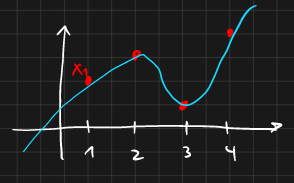
\includegraphics[width=0.25\textwidth]{discrete}\\~\\
Now, vectors become functions $f:{\color{cyan}\mathbb{R}}\rightarrow\mathbb{R}$\\
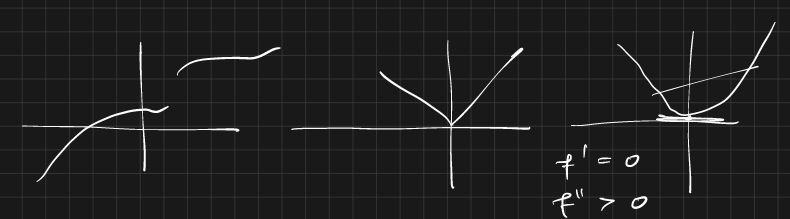
\includegraphics[width=0.75\textwidth]{continuous}

\end{frame}

\begin{frame}
\Subsection{Motivation}
Let us first recall the definition of a linear function. Consider a function $f:\mathbb{R}^n\rightarrow\mathbb{R}^m$, then
$$
f~\text{linear}~:\stackrel{\text{Def}}{\Leftrightarrow}~\forall~x,y\in\mathbb{R}^n,~\lambda\in\mathbb{R}:~f(\lambda\cdot x+y)=\lambda\cdot f(x)+f(y).
$$
The prototype of a linear function between finite dimensional spaces is the matrix--vector product, more precisely,
$$
A\in\mathbb{R}^{m\times n},~f_A(x):=Ax.
$$
{\color{defgruen}We say $f$ is \textbf{nonlinear}, if it is not linear.}
~\\
Nonlinear function may extend our modeling choice significantly and may help to explain complicated relations, such as
$$
\begin{matrix}
z_i&\rightarrow&y_i\\
\in\mathbb{R}^p&~&\in\mathbb{R}^q\\
\text{\color{cyan}[image]}&~&\text{\color{cyan}[feature]}
\end{matrix},~i=1,\dots,m.
$$
Until now, we have consider models with \textit{linear} dependency of the parameters:
\begin{align*}
f_x(z)=\sum_{k=1}^nx_k\cdot f_k(z)\approx y.
\end{align*}
We determined the parameters $x=(x_k)_k$ by solving a (potentially regularized) least squares problem of the form
$$
\min_x L(x;(z_i,y_i))+R(x),~~~\left(\text{e.g., Ridge Regression}~R(x):=\frac{\delta}{2}\|x\|_2^2~\right),
$$
where the cost function has the form
$$\sum_{i=1}^m\|f_x(z_i)-y_i\|_2^2=\|A_zx-y\|_2^2=:L(x,(z_i,y_i)).$$
The specialty of this kind of minimization problem is that we can solve it via the normal equation, which is a \textit{linear} equation.
\end{frame} 

\begin{frame}
Now let us consider a \textbf{nonlinear model} (e.g. Neural Network); more precisely, nonlinear with respect to the sought-after parameters. More specifically, let us for example consider a model of the form
\begin{align*}
f_x(z)=(f_M\circ\dots\circ f_1)(z)=f_M(f_{M-1}(f\dots(f_1(z))\dots))
\end{align*}
where the building blocks $f_k$, also called \textbf{layers}, are given by
$$f_k\colon \R^p \to  [0,+\infty)^q, ~~f_k(z):=(A_kz+b_k)_+~~~\textit{(applied element-wise)},$$ 
with
$$\R\to [0,+\infty), ~~w_+:=\begin{cases} 
0:w<0\\w:~\text{else}
\end{cases}$$
being the so-called \textbf{\href{https://en.wikipedia.org/wiki/Rectifier_(neural_networks)}{ReLU function}} (Rectified Linear Unit), an example of a so-called \textbf{activation function}.\\~\\ 
The matrices $A_k \in \R^{q\times p}$ and vectors $b_k \in \R^{q}$ are the parameters (also called \textbf{weights}) that need to be determined. If $A_k$ is dense, the function $f_k$ is called \text{fully connected layer} and if, e.g., $A_k$ is Toeplitz, then $f_k$ is called \textbf{convolutional layer}.~\\~\\
Due to the ReLU function $(\cdot)_+$ the concatenated model $f_x$ is highly nonlinear.\\
~\\
Similarly to the linear case, we aim to find suitable parameters/weights $x:=(A_k,b_k)_k$ that best describe the model with respect to a certain cost function:
$$
\min_{x:=(A_k,b_k)_k} L(x;(z_i,y_i))+R(x)=:F(x)~~~~~(\leftarrow~\text{$F$ highly nonlinear})
$$

\end{frame}

\begin{frame}
~\\
Before we continue with some standard definitions from calculus, a preliminary remark:
~\\~\\

The concepts of continuity and differentiability in the context of a function $f:\mathbb{R}^n\rightarrow\mathbb{R}^m$  are ``local'' concepts, i.e., they are required to hold in a small neighborhood of a point $x_0\in\mathbb{R}^n$.\\~\\
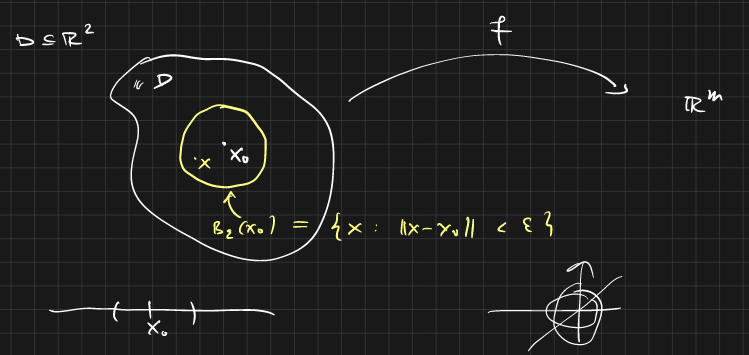
\includegraphics[width=.75\textwidth]{locality}

\end{frame}

\begin{frame}
\Subsection{Continuity and Differentiability}
In the following we consider neighborhoods of the form $B_\varepsilon (x_0):= \{x\in \Rn\colon  \|x-x_0\|< \varepsilon\}$.
\begin{definition}[Continuous and differentiable function]~\\
	Let $D\subseteq\mathbb{R}^n,~f:D\rightarrow\mathbb{R}^m$ and $x_0\in D$ with $B_\varepsilon (x_0)\subseteq D$ for some $\varepsilon>0$. Then
	~\\~\\
	\begin{itemize}
		\item [i)] 
		$f$ is called \textbf{continuous} at $x_0$, if
		$$
		\lim_{n\to 0}\|f(x_n)-f(x_0)\|_2=0
		$$
		for all sequences $(x_n)_{n\in\mathbb{N}}\subseteq B_\varepsilon (x_0)$ for which $x_n\to x_0$.
		
		~\\
		\item [ii)]
		$f$ is called \textbf{differentiable} at $x_0$, if there is a linear mapping $A:\mathbb{R}^n\rightarrow\mathbb{R}^m$ such that
		$$
		\lim_{n\to\infty}\frac{\|(f(x_0)+Ah_n)-f(x_0+h_n)\|}{\|h_n\|}=0
		$$
		for all sequences $(h_n)_n$ with $x_0+h_n\subseteq B_\varepsilon (x_0),~\lim_{n\to\infty}\|h_n\|\to 0$.
		~\\
		Since the linear function $A$ depends on $f$ and $x_0$, we denote it as $Df(x_0):=A$ and call it (Fr\'{e}chet) derivative.
	\end{itemize}
~\\
	If $f$ is continuous/differentiable at any point $x_0\in D$, we call $f$ simply  continuous/differentiable.
\end{definition}
\end{frame}

\begin{frame}
~\\
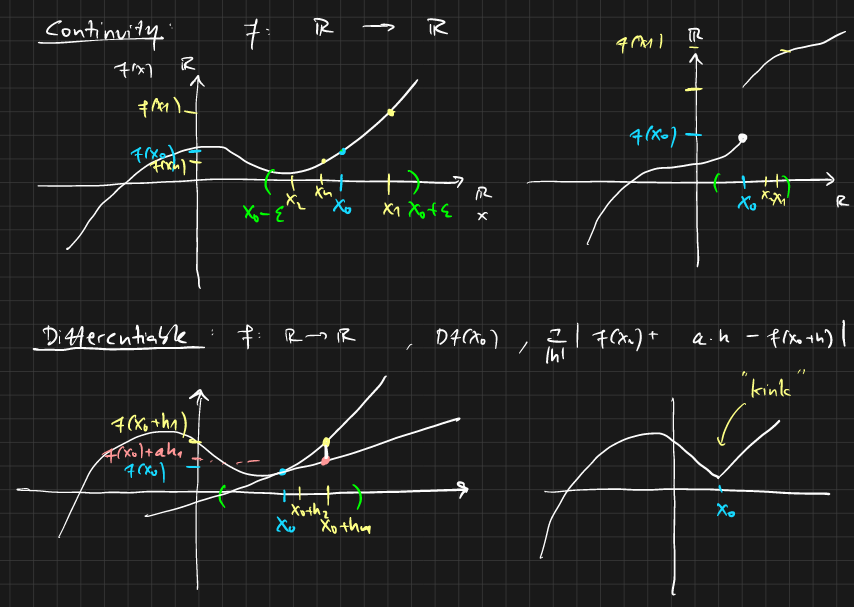
\includegraphics[width=.9\textwidth]{continuous_diff}
\end{frame}

\begin{frame}
\textbf{Examples:} Continuity\\~\\
\begin{itemize}
	\item [i)]
	$f:\mathbb{R}\rightarrow\mathbb{R},~x\mapsto |x|=\begin{cases}
	x:~x\geq 0\\
	-x:~x<0
	\end{cases}$\\~\\
	{\color{cyan}
	Let $x_0\in\mathbb{R},~(x_n)_{n\in\mathbb{N}},~x_n\xrightarrow{n\to\infty}x_0$, then
	$$
	0\leq |f(x_n)-f(x_0)|=||x_n|-|x_0||\leq|x_n-x_0|\xrightarrow{n\to 0} 0
	$$
	$\Rightarrow~~f$ is continuous.
	}
~\\~\\
	\item [ii)]
	$f:\mathbb{R}\rightarrow\mathbb{R},~x\mapsto x^2$\\
	{\color{cyan}
	Let $x_0\in\mathbb{R},~x_n\rightarrow x_0$, then
	$$
	|f(x_n)-f(x_0)|=|x_n^2-x_0^2|=|(x_n-x_0)(x_n+x_0)|=\underbrace{|x_n-x_0|}_{\to 0}\underbrace{|x_n+x_0|}_{\to 2x_0}\xrightarrow{n\to\infty} 0
	$$
	$\Rightarrow~~f$ is continuous.
	}
~\\~\\
	\item [iii)]
	$f:\mathbb{R}\rightarrow\mathbb{R},f(x):=\begin{cases}
	1:~x>0\\
	-1:~x\leq0
	\end{cases}$\\~\\
	{\color{cyan}
	Let $x_0=0,~x_n\rightarrow 0^+$, then
	$$
	|f(x_n)-f(x_0)|=|1-(-1)|=2\nrightarrow 0
	$$
	$\Rightarrow~~f$ is not continuous.
	}
\end{itemize}

\end{frame}

\begin{frame}
	\textbf{Examples:} Differentiability~\\~\\
	\begin{itemize}
		\item [i)]
		$f:\mathbb{R}\rightarrow\mathbb{R},~x\mapsto ax,~a\in\mathbb{R}$ \\~\\
		{\color{cyan}
			Let us consider the surrogate $Df(x_0)(h):=ah$ and a sequence $h_n\to 0$. Then
			\begin{align*}
			&\frac{1}{|h_n|}|f(x_0)+Df(x_0)h_n-f(x_0+h_n)|=\frac{1}{|h_n|}|ax_0+ah_n-a(x_0+h_n)|=0\xrightarrow{n\to\infty} 0
			\end{align*}
			$\Rightarrow~~f$ is differentiable.\\
		}
	~\\~\\
		\item [ii)]
		$f:\mathbb{R}^n\rightarrow\mathbb{R}^m,~x\mapsto Ax,~A\in\mathbb{R}^{m\times n}$\\~\\
		{\color{cyan}
			Let us consider the surrogate $Df(x_0)(h):=Ah$ and a sequence $h_n\to 0$. Then
			\begin{align*}
			&\frac{1}{|h_n|}|f(x_0)+Df(x_0)h_n-f(x_0+h_n)|=\frac{1}{|h_n|}|Ax_0+Ah_n-A(x_0+h_n)|=0\xrightarrow{n\to\infty} 0
			\end{align*}
			$\Rightarrow~~f$ is differentiable.
		}
	~\\~\\
		\item [iii)]
		$f:\mathbb{R}\rightarrow\mathbb{R},~x\mapsto |x|$\\~\\
		{\color{cyan}
			$f$ is \textbf{not} differentiable at $x_0=0$.
		}
	\end{itemize}
\end{frame}

\begin{frame}
\textbf{Remark:} How can we identify continuous/differentiable functions?\\~\\
\begin{itemize}
	\item 
	Many elementary functions (polynomials, trigonometric functions, exponential function,...) and operations (``+'',``$\cdot$'',...) to combine such elementary functions are continuous/differentiable.\\~\\
	\item
	The concatenation of such functions is also continuous/differentiable!\\~\\
	\item Examples:
	\begin{align*}
	&\text{-- monomial}~x^k~~\text{and polynomial (=linear combination)}~~p(x)=\sum_{j=0}^m a_j x^j\\
	&\text{-- expotential function~}~e^x~~\text{and sine function}~\sin(x)=\frac{1}{2i}(e^{ix}-e^{-ix})
	\end{align*}
\end{itemize}
~\\~\\~\\
We will show in the exercise that differentiability is a stronger requirement than continuity:
\begin{theorem}
	Every differentiable function is also continuous.
\end{theorem}
\end{frame}


\begin{frame}
Next, we introduce the directional derivative which often serves as a good starting point to find the (Fréchet) derivative  of a function (especially in complex and confusing situations):

\begin{definition}[Directional derivative]
	We assume that $f:\mathbb{R}^n\rightarrow\mathbb{R}^m$ is (Fr\'{e}chet-) differentiable at $x_0\in\mathbb{R}^n$ with derivative $Df(x_0)$. For a $v\in\mathbb{R}^n$, the limit
	$$
	Gf(x_0)(v):=\lim_{t\to 0^+}\frac{f(x_0+tv)-f(x_0)}{t}
	$$
	exists and it concides with the Fr\'{e}chet derivative, i.e., $Gf(x_0)(v)=Df(x_0)(v)$.\\
	We call $Gf(x_0)(v)$ the \textbf{directional derivative} at $x_0$ in the direction $v$. (G\^{a}teaux derivative)
\end{definition}
~\\
\textbf{Remark:}\\
The G\^{a}teaux derivative may exist, even if $f$ is not Fr\'{e}chet differentiable (e.g. $x\mapsto |x|,~x_0=0$).\\
%However, we note that it is a very convenient way to determine analytical derivatives .\\
%~\\

\end{frame}

\begin{frame}
~\\
\textbf{Examples:}\\~\\
\begin{itemize}
	\item [i)]
	$f:\mathbb{R}\rightarrow\mathbb{R},~x\mapsto |x|,~x_0=0$ (not Fr\'{e}chet-differentiable)\\~\\
	{\color{cyan}
	\begin{itemize}
		\item [\color{cyan}a)]\color{cyan}
		$v\geq 0:~Gf(x_0)(v)=\lim_{t\to 0^+}\frac{1}{t}(f(x_0+tv)-f(x_0))=\lim_{t\to 0^+}\frac{1}{t}(tv)=1\cdot v$
		\item [\color{cyan}b)]\color{cyan}
		$v<0:~Gf(x_0)(v)=\lim_{t\to 0^+}\frac{1}{t}(\underbrace{f(x_0+tv)}_{=-tv}-f(x_0))=(-1)\cdot v$
	\end{itemize}
}
~\\~\\
	\item [ii)]
	$f:\mathbb{R}^n\rightarrow\mathbb{R},~x\mapsto \|x\|_2^2=x^Tx,~v\in\mathbb{R}^n,~x_0\in\mathbb{R}^n$
	{\color{cyan}
	\begin{align*}
	Gf(x_0)(v)&=\lim_{t\to 0^+}\frac{f(x_0+tv)-f(x_0)}{t}\\
	&=\lim_{t\to 0^+}(\underline{(x_0+tv)^T(x_0+tv)}_{x_0^Tx_0+2tx_0^Tv+t^2v^Tv}-x_0^Tx_0)\frac{1}{t}\\
	&=(2x_0)^Tv
	\end{align*}
	Consider $v=\sum_{j=1}^n v_je_j,$ where $e_1,\dots,e_n$ denote the standard basis in $\mathbb{R}^n$, then
	$$
	Df(x_0)(v)=\sum_{j=1}^n v_j\underbrace{\underbrace{Df(x_0)}_{\mathbb{R}^n\to\mathbb{R}^m}(e_j)}_{\in\mathbb{R}^m}
	$$
	}
\end{itemize}

\end{frame}

\begin{frame}
~\\
\begin{definition}[Partial derivative]
	Let $f:D\rightarrow\mathbb{R}^m,~D\subseteq\mathbb{R}^n$ be (Fréchet-)differentiable in $x_0\in D$. We define the so-called \textbf{partial derivatives} of $f$ at $x_0$ with respect to the j-th variable by:
	$$
	\frac{\partial}{\partial x_j}f(x_0):=Df(x_0)(e_j),
	$$
	where $e_j$ is the j-th standard basis vector.
\end{definition}
{
Now again with $v=\sum_{j=1}^n v_je_j$ we find
\begin{align*}
Df(x_0)(v)&=\sum_{j=1}^n v_j Df(x_0)(e_j)\\
&=\begin{pmatrix}
|&~&|\\
Df(x_0)(e_1)&\cdots&Df(x_0)(e_n)\\
|&~&|
\end{pmatrix}\begin{pmatrix}
v_1\\\vdots\\v_n
\end{pmatrix}\\
&=\begin{pmatrix}
|&~&|\\
\frac{\partial}{\partial x_1}f(x_0)&\cdots&\frac{\partial}{\partial x_n}f(x_0)\\
|&~&|
\end{pmatrix}v\\
&=\underbrace{J_f(x_0)}_{\in\mathbb{R}^{m\times n}}\cdot v\\
&f:\mathbb{R}^n\rightarrow\mathbb{R}^m,~f(x)=\begin{pmatrix}
f_1(x)\\\vdots\\f_m(x)
\end{pmatrix},~f_i:\mathbb{R}^n\rightarrow\mathbb{R}
\end{align*}
}
\end{frame}

\begin{frame}
Since $Df(x_0):\mathbb{R}^n\rightarrow\mathbb{R}^m$ is linear it can be represented by a matrix:
~\\
\begin{lemma}[Jacobian]
Let $f:\mathbb{R}^n\supset D\rightarrow\mathbb{R}^m$ be differentiable at $x_0\in D$ with derivative $Df(x_0):\mathbb{R}^n\rightarrow\mathbb{R}^m$. Then the so-called \textbf{Jacobian matrix}
$$
J_f(x_0):=\mathcal{M}_{I}^{I}(Df(x_0)) =\begin{pmatrix}
\frac{\partial f_1}{\partial x_1}(x_0)&\cdots&\frac{\partial f_1}{\partial x_n}(x_0)\\\vdots&\ddots&\vdots\\
\frac{\partial f_m}{\partial x_1}(x_0)&\cdots&\frac{\partial f_m}{\partial x_n}(x_0)
\end{pmatrix}\in\mathbb{R}^{m\times n}
$$
is the matrix representation of $Df(x_0)$ with respect to the standard bases in $\Rn$ and $\Rm$.
\end{lemma}
~\\~\\
In the special case, that the Jacobian matrix is just one row we give it a special name:
\begin{definition}[Gradient]
	Let $f:\mathbb{R}^n\supset D\rightarrow\mathbb{R}$ be differentiable at $x_0\in D$, then
	$$
	J_f(x_0)^T=\begin{pmatrix}
	\frac{\partial f}{\partial x_1}(x_0)\\
	\vdots\\
	\frac{\partial f}{\partial x_n}(x_0)
	\end{pmatrix}=:\nabla f(x_0)
	$$
	is called the \textbf{gradient of $f$} at $x_0\in D$.
\end{definition}
\end{frame}

\begin{frame}
~\\~\\
\textbf{Example}~\\~\\
\Hide{
Let us again consider $f:\mathbb{R}^n\rightarrow\mathbb{R}$ with
$$~x\mapsto x^Tx=\sum_{i=1}^n x_i^2=x_1^2+x_2^2+\dots+x_n^2.$$
Then
\begin{align*}
\frac{\partial f}{\partial x_i}(x)&=2 x_i\\
\nabla f(x)&=2\begin{pmatrix}
x_1\\\vdots\\x_n
\end{pmatrix}=2x\\
Df(x)(v)&=(2x)^Tv\\
J_f(x)\cdot v&=\nabla f(x)^T\cdot v =(2x)^Tv
\end{align*}
}
\end{frame}

 
 

\begin{frame}
\Subsection{Solving Nonlinear Equations: Taylor Approximation and Newton's Method}
The next result is on the approximation quality of the derivative:
\begin{lemma}[Taylor approximation]\label{taylor}
Let $f:\R^n\supset B_\varepsilon(\hat{x})\to\R^n$ be differentiable at $\hat{x}$ with some $\varepsilon>0$. Assume further that there is a (Lipschitz) constant $L \geq 0$ such that the Jacobian  $J_f$
satisfies
\begin{align}
\|J_f(y)-J_f(x)\|\le L\|y-x\|\, ,\quad\forall x,y\in B_\varepsilon(\hat{x}). \label{lipschitz}
\end{align}
Then, there holds
$$
\|f(y)-\left[f(x)+J_f(x)(y-x)\right]\|\le \frac{L}{2}\|y-x\|^2\, ,\quad\forall x,y\in B_\varepsilon(\hat{x})
$$
which we rephrase with the notation:
$$
f(y)=f(x)+J_f(x)(y-x) + \mathcal{O}(\|y-x\|^2).
$$
\end{lemma}
~\\
Let us apply Taylor approximation to solve nonlinear systems: The idea is to locally approximate the nonlinear function by its linear derivative and then solve many linear systems.\\ ~\\
\begin{itemize}
	\item \underline{Situation:} Consider for a potentially nonlinear function $f:\mathbb{R}^n\rightarrow\mathbb{R}^n$ and the nonlinear system $f(\hat{x})=0$\\
%~\\
\item \underline{Aim:} Determine the solution $\hat{x}$ (iteratively/numerically)\\
%~\\
\item \underline{Idea:} Define an iterative scheme $~x^{k+1}:=x^k+\Delta x^k$ where the increment is derived as follows:
\begin{align*}
0\stackrel{!}{=}f(x^{k+1})&=f(x^k+\Delta x^k)\approx f(x^k)+J_f(x^k)\Delta x^k~~(\rightsquigarrow~\text{solve for}~\Delta x^k)\\
\Leftrightarrow~~J_f(x^k)\cdot \Delta x^k&=-f(x^k)~~~~~(\text{linear equation})\\
\Leftrightarrow~~\Delta x^k&=-J_f(x^k)^{-1}f(x^k)~~~~~(\text{invertibility of the derivative at each $x_k$ assumed!})\\
x^k&\rightarrow\hat{x}
\end{align*}
\end{itemize}
\end{frame}


\begin{frame}
~\\
One can show the following convergence result of this approach:
%NEWTON_KANTOROVICH
\begin{theorem}[simplified Newton-Kantorovich]
	Let $f:\R^n\supset B_\varepsilon(\hat{x})\to\R^n$ be differentiable with invertible derivative for some $\varepsilon>0$ and $f(\hat{x})=0$. Assume the Lipschitz condition \eqref{lipschitz} and the existence of an upper bound $\|J_f(x)^{-1}\|<M$ for some $M<\infty$ and for all $x\in B_\varepsilon(\hat{x})$. Then, the Newton iteration
	\[
	\boxed{x^{k+1}:=x^k+\Delta x^k\, , \text{~ where~ }\Delta x^k\text{~ solves~ }f(x^k)+J_f(x^k)\Delta x^k=0}
	\]
	converges quadratically to $\hat{x}$, provided $x^1$ is chosen sufficiently close to $\hat{x}$, i.e.
	\[
	\|x^{k+1}-\hat{x}\|\le c \|x^{k}-\hat{x}\|^2\, ,\quad c<\infty.
	\]
\end{theorem}

~\\~\\
\textbf{Remark}\\
In many cases, Newton's method does not work right out of the box, because the starting vector $x^1$ is too far away from the solution. Then, techniques for adaptive step-length reduction (damping, relaxation, line-search) have to be used in order to enforce convergence. Details of these approaches fill multiple books. When Newton's method works, i.e., after an initial damped phase, it gets super fast.
\end{frame}



\begin{frame}[c]
~\\
{
\textbf{Take-away messages:}\\~\\
\begin{itemize}
	\item Derivatives $\rightarrow$ local linear approximation to the function
	\item Newton's method $\rightarrow$ solves nonlinear systems by solving many linear problems in each step
\end{itemize}
}

\end{frame}

\begin{frame}
	\Subsection{The Chain Rule and Back Propagation}
	The chain rule lies at the heart of back propagation. It tells us how to compute the  derivative of concatenated functions:
	\begin{theorem}[Chain rule] \label{chain}Consider mappings $g:\R^\ell\supset D_g\to D_f\subset\R^m$ differentiable in $x_0\in D_g$ with Jacobian $J_g(x_0)$ and $f:\R^m\supset D_f\to \R^n$, differentiable in $g(x_0)\in D_f$ with Jacobian $J_f(g(x_0))$. Then, the concatenation is differentiable with Jacobian $J_{f\circ g}(x_0)$ and
		\[
		D(f\circ g)(x_0)=Df(g(x_0))\circ Dg(x_0)\text{~~~and~~~}
		\boxed{J_{f\circ g}(x_0)=J_f(g(x_0))\cdot J_g(x_0)}.
		\]
	\end{theorem}
\begin{example}
	Let us revisit our regularizer from the imaging example:\\
	Consider $D\in \R^{p \times n}$ and the linear function $g\colon\Rn \to \R^p, ~g(x):= Dx$. Then for all $x\in\Rn$ we easily find
	$$J_g(x) = D.$$
	Also, let $f\colon \R^p \to \R,~f(y):=\tfrac{1}{2}y^\top y = \tfrac{1}{2} \|y\|_2^2$, then we have seen above that, for all $y\in\R^p$,
	$$J_f(y)^\top = \nabla f(y) = \tfrac{1}{2}2y=y. $$
	Then the concatenation $h := (f\circ g): \Rn \to \R$ is given by
	$$h(x) = \tfrac{1}{2} \|Dx\|_2^2 $$
	with gradient, at $x\in \Rn$, obtained from the chain rule
	$$\nabla h(x) = J_h(x)^\top = \left(J_f(g(x))\cdot J_g(x) \right)^\top = D^\top \nabla f(g(x)) = D^\top  g(x) = D^\top Dx. $$
\end{example}
\end{frame}

%
%\emph{Simple first example:} Consider concatenated differentiable functions $f\circ g(x)$ written in the seemingly complicated form with intermediate variable $z$:
%\[
%f(z)\text{ , where }z-g(x)=0 
%\]
%Thus, $z$ is a function of $x$, namely $z(x)=g(x)$. Thus,
%\[
%f\circ g(x)\equiv\LL(x,\lambda):= f(z(x))+\lambda^\top(z(x)-g(x))\, ,
%\text{ for any }\lambda.
%\]
%Now,
%\begin{align*}
%\frac{d(f\circ g)(x)}{dx}&=
%\frac{\partial \LL(x,\lambda)}{\partial x}=
%\frac{df}{dz}\frac{dz}{dx}+\lambda^\top\left(\frac{dz}{dx}-\frac{dg}{dx}\right)\\
%&=\left(\frac{df}{dz}+\lambda^\top\right)\frac{dz}{dx}-\lambda^\top\frac{dg}{dx}
%\end{align*}
%Thus, $d(f\circ g)/dx$ can be determined in two steps (note that $\lambda$ can be chosen arbitrarily)
%\ite
%\item[(1)] $\lambda:=-\left(\frac{df}{dz}(z(x))\right)^\top$
%\item[(2)] $\frac{d(f\circ g)(x)}{dx}=-\lambda^\top\frac{dg}{dx}(x)
%$
%\eti
%
%These two steps are just a more complicated formulation of the chain rule, but this Lagrangian principle is the foundation of the backward mode of automatic differentiation and also of the back propagation in ANN, as we'll see now.
%
%\emph{Abstract back propagation:}
%We consider the concatenation
%\begin{align*}
%h(w_N,\ldots, w_1,x):=&f(g_N(w_N,(g_{N-1}(w_{N-1},(\ldots ,g_1(w_1,x))\ldots ))))\\
%=&f\circ g_{N}(w_{N},\cdot)\circ g_{N-1}(w_{N-1},\cdot)\circ\cdots
%\circ g_{1}(w_{1},x)
%\end{align*}
%illustrated by the diagramm:
%
%\hspace{0.5cm}
%\begin{tikzpicture}[->,>=stealth',shorten >=1pt,auto,node distance=2.2cm,
%semithick]
%\node (input) at (0,0){$x$};
%\node (g1) at (2,0){\fbox{$g_{1}$}};
%\node (w1) at (2,-1.5){$w_1$};
%\node (z1) at (4,0){$z_{1}$};
%\node (gNm1) at (7,0){\fbox{$g_{N-1}$}};
%\node (wNm1) at (7,-1.5){$w_{N-1}$};
%\node (zNm1) at (9.25,0){$z_{N-1}$};
%\node (gN) at (11.25,0){\fbox{$g_N$}};
%\node (wN) at (11.25,-1.5){$w_N$};
%\node (zN) at (13.25,0){$z_N$};
%\node (fz) at (15.25,0){$f(z_N)$};
%\draw[->] (input) -- (g1);
%\draw[->] (w1) -- (g1);
%\draw[->] (g1) -- (z1);
%\draw[->, dotted] (z1) -- (gNm1);
%\draw[->] (wNm1) -- (gNm1);
%\draw[->] (gNm1) -- (zNm1);
%\draw[->] (zNm1) -- (gN);
%\draw[->] (wN) -- (gN);
%\draw[->] (gN) -- (zN);
%\draw[->] (zN) -- (fz);
%\end{tikzpicture}
%
%
%Again, this can be written in the fashion
%\[
%h(w_N,\ldots, w_1,x)=f(z_{N})\text{ ,~ where~ }z_k-g_k(w_k,z_{k-1})=0\, , ~~~k=1,\ldots,N\, , ~~z_0:=x
%\]
%Again
%\[
%h(w_N,\ldots, w_1,x)\equiv
%\LL(w,x,\lambda):=f(z_N)+\sum_{k=1}^N\lambda_k^\top(z_k-g_k(w_k,z_{k-1}))\, ,
%\text{~~ for any }\lambda_k
%\]
%Thus
%\begin{align*}
%\frac{dh}{dw_i}&=\frac{df}{dz}\frac{dz_N}{dw_i}+
%\sum_{k=i}^N\lambda_k^\top\frac{dz_k}{dw_i}-\sum_{k=i+1}^N\lambda_k^\top\frac{\partial g_k}{\partial z}\frac{\partial z_{k-1}}{\partial w_i} -\lambda_i^\top\frac{\partial g_i}{\partial w_i}\\
%&=\frac{df}{dz}\frac{dz_N}{dw_i}+
%\sum_{k=i}^N\lambda_k^\top\frac{dz_k}{dw_i}-\sum_{k=i}^{N-1}\lambda_{k+1}^\top\frac{\partial g_{k+1}}{\partial z}\frac{dz_{k}}{dw_i} -\lambda_i^\top\frac{\partial g_i}{\partial w_i}\\
%&=\left(\frac{df}{dz}+\lambda_N^\top\right)\frac{dz_N}{dw_i}+
%\sum_{k=i}^{N-1}\left(\lambda_k^\top-\lambda_{k+1}^\top\frac{\partial g_{k+1}}{\partial z}\right)\frac{dz_{k}}{dw_i} -\lambda_i^\top\frac{\partial g_i}{\partial w_i}.
%\end{align*}
%Thus, if the $\lambda$'s satisfy the recursion
%\[
%\lambda_N=-\left(\frac{df}{dz}(z_N)\right)^\top\, ,\ 
%\lambda_k=\left(\frac{\partial g_{k+1}}{\partial z}(w_{k+1},z_k)\right)^\top \lambda_{k+1}\, ,\qquad 
%k=N-1,N-2,\ldots, i
%\]
%we achieve the expression
%\[
%\frac{dh}{dw_i}(w_N,\ldots, w_1,x)= -\lambda_i^\top\frac{\partial g_i}{\partial w_i}(w_i,z_{i-1}).
%\]
%
%\begin{remark}
%	The technique presented is an example of a fairly general principle for the derivation of iterations towards complicated derivatives. This principle is used in the backward mode of automatic differentiation and in the derivation of adjoint equations for optimization problems involving differential equations.
%\end{remark}
%
%
%
%\begin{frame}
%	\Subsection{Integration and quadrature}
%
%Quadrature = numerical approximation of an integral  
%
%Here, we do not go very deep into the foundations, but rather use the following operational definition. A more detailed view is required for measure and probability theory.
%\gbegin{definition}\label{def-integral} ~\\[-0.7cm]
%\ite
%\item[(1D)] For the interval $[a,b]$ with $-\infty< a\le b<\infty$ and an (integrable) function $f:[a,b]\to\R$, we define
%\[
%\int_a^bf(x)dx:=F(b)-F(a)=:[F(x)]_a^b\, , \text{ where } F:[a,b]\to\R \text{ satisfies } F'(x)=f(x) 
%\]
%If instead $f:[a,b]\to\R^k$, this definition is applied to each component $f_i(x)$ separately.
%\item[(nD)] Consider a domain $D:=\mathop{\times}_{i=1}^n[a_i,b_i]$  with $-\infty< a_i\le b_i<\infty$ and an (integrable) function $f:D\to\R^k$. We define
%\[
%\int_D f(x)dx:=\int_{a_1}^{b_1}\int_{a_2}^{b_2}\ldots\int_{a_n}^{b_n}
%f(x_1,x_2,\ldots,x_n)dx_n\ldots dx_2dx_1
%\]
%\eti
%If $a,b$ or $a_i,b_i$ are not finite or if $f$ is not finite there, one has to use appropriate limits. A function $f$ is called \textbf{integrable}, if the expressions defined above are well defined and finite. Countably many points on $\R$ are considered zero sets and integrals over them are zero per definition.
%\bend{definition}
%\end{frame}
%
%\begin{frame}
%	\newpage 
%{
%	\blank
%	\small
%	~ \\[-1.5cm]
%	\begin{bsp} 
%		\begin{itemize}
%			\item[a)] \[\int\limits_0^1 x^3 dx = [\frac{x^4}{4}]_0^1 = \frac{1}{4}\]   \\[-0.9cm]
%			\item[b)] \[\int_D \norm{x}^2 dx = \int_{[0,1]^2} x^\top x dx = \int_0^1 \int_0^1 (x_1^2 +x_2^2) dx_1 dx_2 = 
%			\int_0^1 [\frac{x_1^3}{3} + x_1 x_2^2]_0^1 dx_2 = \int_0^1 \frac{1}{3} + x_2^2 dx_2 = [\frac{x_2}{3} + \frac{x_2^3}{3}]^1_0 = \frac{1}{3}+\frac{1}{3} = \frac{2}{3}\]
%		\end{itemize}
%	\end{bsp}
%	\textbf{Substitution rule in 1d} \vspace{-0.5cm}
%	\begin{itemize}
%		\item[] \[ \int_a^b f(x) dx,\; \text{let}\; x = g(y) \Rightarrow \frac{dx}{dx} = g^\prime (y) \Rightarrow dx = g^\prime (gy) dy \]
%		\item[] \[ \Rightarrow \exists \alpha,\beta \; \text{with}\; a=g(\alpha), b= g(\beta): \hspace{0.5cm} \int_a^b f(x) dx = \int_\alpha^\beta f(g(y))g^\prime (y) dy \]
%	\end{itemize}
%	\begin{bsp}
%		\begin{itemize}
%			\item[] \[ \int_{1/50}^2 \frac{e^{\frac{2}{y}}}{y^2}dy, \; \text{let}\; x := \frac{2}{y} = 2\cdot y^{-1}\]
%			\item[] \[ \Rightarrow \frac{dx}{dy} = - \frac{2}{y^2} \Rightarrow \frac{1}{y^2} dy = - \frac{dx}{2} \; \text{and} \; a = \frac{2}{1/50} = 100, b= \frac{2}{2} = 1\]
%			\item[] \[ \Rightarrow \int_{1/50}^2 \frac{e^{\frac{2}{y}}}{y^2}dy = \int_{1/50}^2 e^{\frac{2}{y}} \underbrace{\frac{1}{y^2}dy}_{-\frac{dx}{2}} = \int_100^1 - \frac{e^x}{2}dx = -\frac{1}{2}(e^1 - e^{100}) = \frac{e^{100}-e^1}{2}\]
%		\end{itemize}
%	\end{bsp}
%}
%\end{frame}
%
%
%
%\begin{frame}
%	{
%	\blank
%	\textbf{Substitution rule in nD:}
%	\begin{itemize}
%		\item[] \[ \int_D f(x)dx, \; \text{let}\; x=g(y), g \; \text{invertible (on image) and} \]
%		\item[] \[ D = g(E) \Rightarrow dx = \sqrt{\det(Dg(y)^\top Dg(y))}dy\] 
%		\item[] \[ \int_D f(x)dx = \int_E f(g(y))\sqrt{\det(Dg(y)^\top Dg(y))}dy\]
%	\end{itemize}
%	\begin{bsp}
%		\begin{itemize}
%			\item[a)]\begin{itemize}
%				\item[] $\left(\begin{array}{c}
%				x_1\\
%				x_2
%				\end{array}\right) = g \left(\begin{array}{c}
%				r\\
%				\phi
%				\end{array}\right) = \left(\begin{array}{c}
%				r \cos{\phi}\\
%				r \sin{\phi}
%				\end{array}\right)$\\
%				\item[] $Dg = \begin{bmatrix}
%				\frac{\partial g_1}{\partial r} & \frac{\partial g_1}{\partial \phi}\\
%				\frac{\partial g_2}{\partial r} & \frac{\partial g_2}{\partial \phi}
%				\end{bmatrix} = \begin{bmatrix}
%				\cos{\phi} & -r\sin{\phi} \\
%				\sin{\phi} & r\cos{\phi}
%				\end{bmatrix}$\\
%				\item[] $\abs{\det(Dg)} = \abs{\cos{\phi r}\cos{\phi} - \sin{\phi}(-r\sin{\phi})} = \abs{r(\cos{\phi}^2 + \sin{\phi}^2)} = r$\\
%				\item[] Area of D = \[ \int_D 1dx = \int_E 1\abs{\det(Dg(r,\phi))}d(r,\phi) = \int_o^\pi \int_1^2 rdrd\phi = \frac{3}{2}\pi\]
%			\end{itemize}
%			\item[b)] Surface of the unit ball\\
%			%		\begin{tikzpicture}[line cap=round, line join=round]
%			%		\clip(-2.19,-2.49) rectangle (2.66,2.58);
%			%		\draw(0,0) circle (2cm);
%			%		\draw [rotate around={0.:(0.,0.)},dash pattern=on 3pt off 3pt] (0,0) ellipse (2cm and 0.9cm);
%			%		\draw [->] (0,0) -- (0,2);
%			%		\draw [->] (0,0) -- (-0.81,-0.79);
%			%		\draw [->] (0,0) -- (2,0);
%			%		\draw (-1.2,-0.75) node[anchor=north west] {$\mathbf {\hat{x}}$};
%			%		\draw (2.07,0.3) node[anchor=north west] {$\mathbf {\hat{y}}$};
%			%		\draw (-0.27,2.6) node[anchor=north west] {$\mathbf {\hat{z}}$};
%			%		\scriptsize
%			%		\end{tikzpicture} 
%			\begin{itemize}\small
%				\item[] $\left(\begin{array}{c}
%				x\\
%				y\\
%				z
%				\end{array} \right) g(\phi,\theta), \hspace{1cm}0 \leq \theta \leq \frac{\pi}{2}, 0 \leq \phi \leq \frac{\pi}{2}$\\
%				\item[] $g(\phi,\theta) = \left(\begin{array}{c}
%				\cos{\phi}\cos{\theta}\\
%				\sin{\phi}\sin{\theta}\\
%				\sin{\theta}
%				\end{array}
%				\right)$\\
%				\item[] $Dg = \begin{bmatrix}
%				-\sin{\phi}\cos{\theta} & -\cos{\phi}\sin{\theta}\\
%				\cos{\phi}\cos{\theta} & -\sin{\phi}\sin{\theta}\\
%				0 & \cos{\theta}
%				\end{bmatrix} \in \mathbb{R}^{3\times2}$\\
%				\item[] $\sqrt{\det(Dg(\phi,\theta)^\top Dg(\phi,\theta)} = \cdots = \cos{\theta}$\\
%				\item[] \[\int_0^1 1 dA = \int_E 1\sqrt{\det(Dg(\phi,\theta)^\top Dg(\phi,\theta))}d\theta d\phi\]
%				\item[] \[ = \int_0^{\frac{\pi}{2}}\int_0^{\frac{\pi}{2}} \cos{\theta}d\theta d\phi = \int_0^{\frac{\pi}{2}}\underbrace{[\sin{\theta}]_0^{\frac{\pi}{2}}}_{1} d\phi = \frac{\pi}{2}\] 
%				\item[] Total surface of unitball = $8 \cdot \abs{0} = 8\cdot \frac{\pi}{2} = 4\pi$
%			\end{itemize}
%		\end{itemize}
%	\end{bsp}
%}
%\end{frame}
%
% 
%\begin{frame}
%	{\bf Idea of numerical integration, aka quadrature:} approximate the function to be integrated piecewise by simple functions, for which the integral is given analytically.
%
%Example: trapezoidal rule:
%
%\pgfplotsset{
%	integral axis/.style={
%		axis lines=middle,
%		enlarge y limits=upper,
%		axis equal image, width=12cm,
%		xlabel=$x$, ylabel=$y$,
%		ytick=\empty,
%		xticklabel style={font=\small, text height=1.5ex, anchor=north},
%		samples=100
%	},
%	integral/.style={
%		domain=2:10,
%		samples=9
%	},
%	integral fill/.style={
%		integral,
%		draw=none, fill=#1,
%		%on layer=axis background
%	},
%	integral fill/.default=cyan!10,
%	integral line/.style={
%		integral,
%		very thick,
%		draw=#1
%	},
%	integral line/.default=black
%}
%
%\hspace{2cm}
%\begin{tikzpicture}[
%% The function that is used for all the plots
%declare function={f=x/5-cos(deg(x*1.85))/2+2;}
%]
%\begin{axis}[
%integral axis,
%ymin=0,
%xmin=0.75, xmax=11.25,
%domain=1.5:10.4,
%xtick={2,...,10},
%xticklabels={$a=x_0$, $x_1$,,,$x_{j-1}$,$x_j$,,$x_{n-1}$,$b=x_n$},
%axis on top
%]
%% The filled area under the approximate integral
%\addplot [integral fill=cyan!15] {f} \closedcycle;
%
%% The highlighted segment
%\addplot [integral fill=cyan!35, domain=6:7, samples=2] {f} \closedcycle;
%
%% The function
%\addplot [very thick, cyan!75!blue] {f} node [anchor=south] {$y=f(x)$};
%
%% The approximate integral
%\addplot [integral line=black] {f};
%
%% The vertical lines between the segments
%\addplot [integral, ycomb] {f};
%
%\end{axis}
%\end{tikzpicture}
%\begin{align*}
%\int_{x_{j-1}}^{x_j}f(x)dx\approx\int_{x_{j-1}}^{x_j}\frac{x_{j-1}-{\color{red}x}}{x_j-x_{j-1}}
%\cdot f(x_{j-1})+\frac{{\color{red}x}-x_{j-1}}{x_j-x_{j-1}}
%\cdot f(x_{j})d{\color{red}x}=(x_j-x_{j-1})\cdot\frac{f(x_{j-1})+f(x_{j})}{2}
%\end{align*}
%Thus, for constant distances $x_j-x_{j-1}\equiv h:=(b-a)/n$, we obtain
%\[
%\int_a^bf(x)dx=\frac{f(a)+f(b)}{2}+\sum_{i=1}^{n-1}h\cdot f(x_i)+\mathcal{O}(h^2) 
%\]
%This can be generalized to higher order polynomials, as well as, to higher dimensions.
%\end{frame}
%
%
%
%
